\chapter{Alternative modeling techniques}

This chapter deals with other possibilities of modeling the technical
system, particularly the double-acting pneumatic piston. Physical modeling
and data-driven modeling methods were examined in terms of suitability for
applying FDI and PdM strategies.

\section{Physical Modeling}
Physical modeling operates with models with a compiled layout that matches
the structure of the different physical domains. In this type of software,
it is possible to combine different domains to create a complex system
model.

Matlab/Simulink provides a physical modeling library, Simscape, that meets
the above specifications. Using Simscape software, the user combines a
model from different blocks representing different physical functions
(spring, resistance, hydraulic valve), and connection links represent some
types of energy flow.



\subsection{The double-acting pneumatic piston modeling in Simscape}

In this part, the same assumption applies as in section \ref{assumptions}. All the
processes take place adiabatically, i.e., without heat exchange with the
environment. 

The resulting model was compiled using gas and mechanical domains \ref{simscape}.

\begin{figure}[h!]
    \centering
    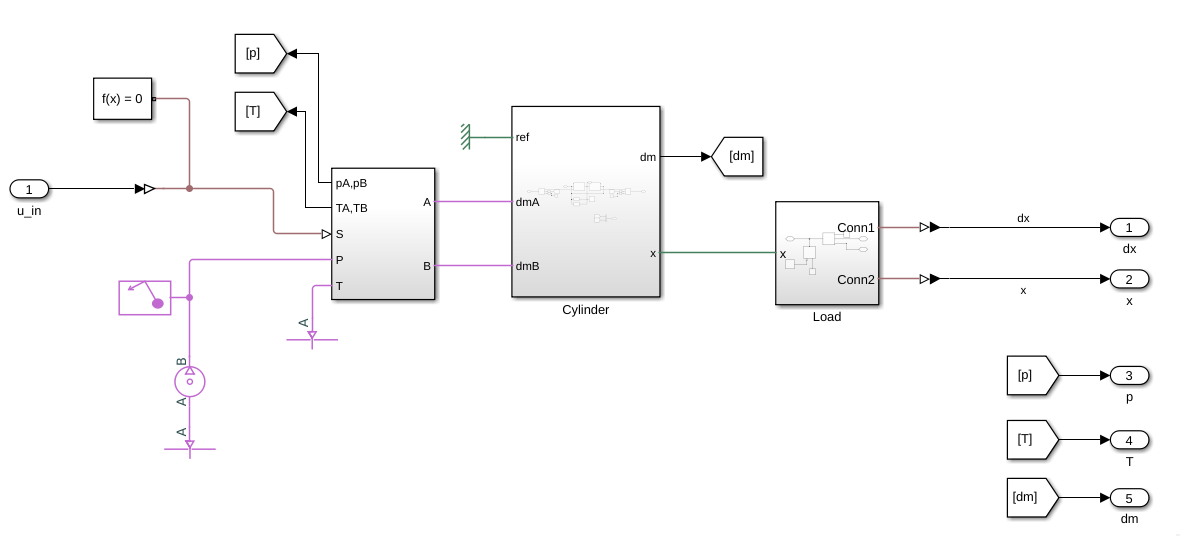
\includegraphics[width=1\textwidth]{simscape.png}
    \caption{The double-acting pneumatic piston developed using Simscape
    software}
    \label{fig:simscape}
\end{figure}


\subsection{Limitations}

It is necessary to know well the parameters of the system.

For example, we need to have a precision-measured characteristic of flow
control valve adjustment in the form of a lookup table to use a throttle
valve block.

Providing simplification and reduce the model to the only control valve,
there are still a few parameters that are not available such as valve and
dampers coefficients mentioned before \ref{}.

The main problem is the computational complexity of the model compared with
the first principle model. During the parameter estimation, the first
principle model is much faster than the Simscape model and gives an option
to experiment with different fault states analysis. 

However, both models showed quite close behavior during testing with the
same parameters; results shown in figure \ref{}.


\section{Data-Driven Models}
Data-Driven modeling explores collected measured signals to identify the
system structure or learn the system behavior from data.

Between data-driven common models belongs parametric and non-parametric
models. Parametric models take part in the system identification field. A
collection of different generalized mathematical models can be fitted to
the input-output signals pair, such as transfer functions, polynomial
models, non-linear ARX models, etc.  A typical representative of
non-parametric models are neural networks of various structures.  In this
thesis, experiments on test datasets were performed with both types of
models. 
\subsection{Hammerstein-Wiener Model}

\begin{figure}[h!]
    \centering
    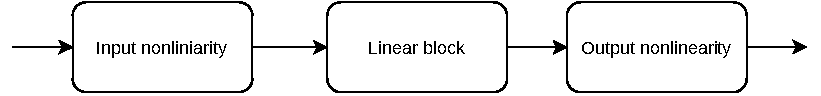
\includegraphics[width=0.7\textwidth]{hw_model.pdf}
    \caption{Hammerstein-Wiener model structure}
    \label{fig:hw_model}
\end{figure}

The best results between parametric models using System Identification
Toolbox, shown Hammerstein-Wiener Model. The model consists of three blocks
\ref{fig:hw_model}, input nonlinearity, linear block and output
nonlinearity.  The nonlinearities are represented by different functions
such as dead-zone, polynomial estimator, saturation, wavelet network
function, etc. 


\begin{figure}[h!]
    \centering
    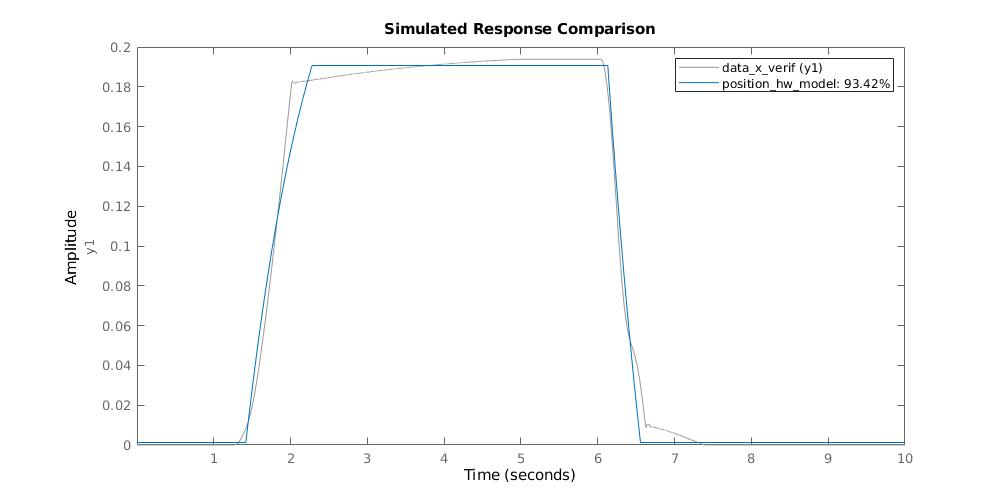
\includegraphics[width=0.8\textwidth]{hw_position.png}
    \caption{Simulated Response for Position Signal Comparison}
    \label{fig:hw_position}
\end{figure}

\begin{figure}[h!]
    \centering
    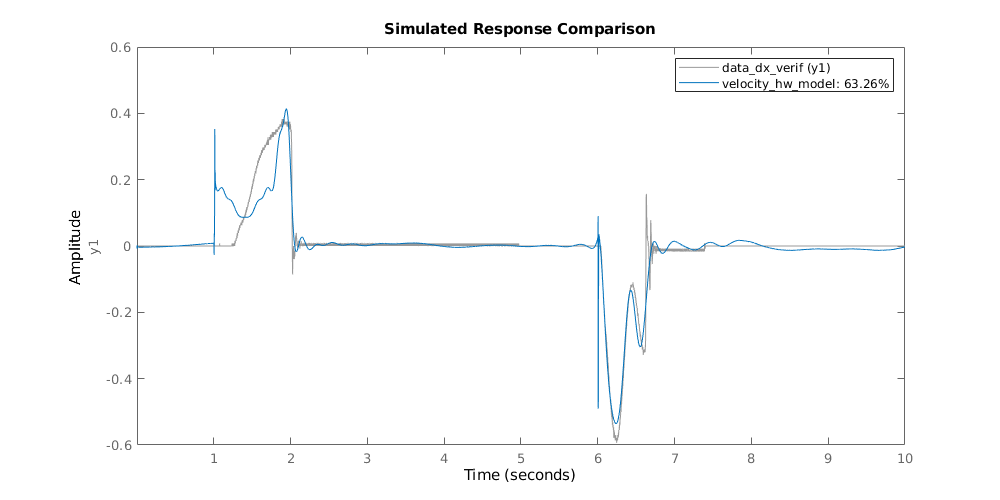
\includegraphics[width=0.8\textwidth]{hw_velocity.png}
    \caption{Simulated Response for Velocity Signal Comparison}
    \label{fig:hw_velocity}
\end{figure}

However, using the identified model, adequate behavior to the measured data
was achieved only for the position signal \ref{fig:hw_position}. The model identified
for velocity signal did not show acceptable behavior \ref{fig:hw_velocity}.  The
reason is the significant nonlinearity and complexity of the system, which
the simplified models cannot take into account.



\newpage
\subsection{NARX Model}

Different structures can be used to train the neural network to predict
system behavior. The most common way is using the nonlinear autoregressive
with the external input model (NARX). This model predicts time-series data
by using different numbers of time-delayed values of input and output
signals \ref{fig:ann}.

\begin{figure}[h!]
    \centering
    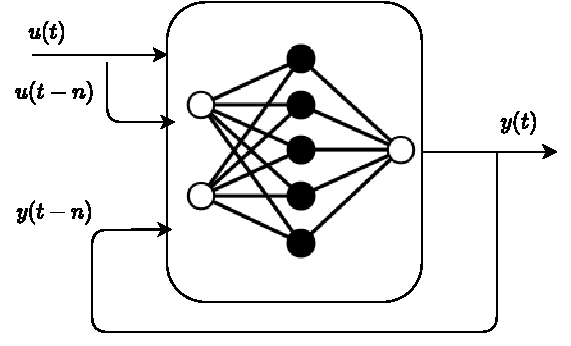
\includegraphics[width=0.5\textwidth]{ann.pdf}
    \caption{Schematical representation of NARX model}
    \label{fig:ann}
\end{figure}


During the development of the model, it is necessary to pay attention to
overfitting, which can significantly impair the performance of the model
and its generalization capabilities.

Some experiments have been performed with this modeling approach. The
Neural Network can predict the behavior of the system based on input.

\subsection{Limitations}
\todo[inline]{Text about only normal behavior}
